\lecture{14}{10 aprile 2024}
\section{Onde vettoriali}
Generalizziamo ora la trattazione delle onde al caso in cui le perturbazioni siano vettoriali. Per quanto riguarda la corda, ad esempio, se ci limitiamo agli spostamenti trasversali nello spazio vediamo che la corda si può muovere sia su y che su z. Le relazioni fra le componenti del vettore e delle sue derivate vanno sotto il nome generico di "polarizzazione". Consideriamo una grandezza generica:
\begin{equation}
	\vec{\xi}(\vec{r},t)=\xi _x(\vec{r},t) \vec{\hat{i}} + \xi _y(\vec{r},t) \vec{\hat{j}} + \xi _z(\vec{r},t) \vec{\hat{k}} 
\end{equation}
L'equazione di D'Alembert non varia, è come se ogni componente si propagasse indipendentemente dalle altre:
\begin{equation}
	\laplacian{\vec{\xi}(\vec{r},t)}=\frac{1}{v^{2} }\frac{\partial ^{2} \vec{\xi}(\vec{r},t)}{\partial t^{2} }  
\end{equation}
che ha per ogni componente la stessa soluzione delle onde scalari. Sembra che non ci siano relazioni fra le componenti! Tuttavia non è così, potrebbero esserci delle equazioni di partenza che collegano le grandezze che si propagano (es: equazioni di Maxwell), oppure potrebbe esserci qualcosa che le correla alla sorgente (es: corda ruotata nel salto della corda).

\subsection{Onde piane vettoriali}
In generale la soluzione è formalmente simile a quella per le onde piane scalari:
\begin{equation}
	\forall \vec{\hat{u}} \forall \vec{f} \in \mathcal{C} ^{2},\ \vec{\xi}(\vec{r},t) = \vec{f}(\vec{\hat{u}} \cdot \vec{r}-vt)
\end{equation}
Per esempio, poniamo \(\vec{\hat{u}}= \vec{\hat{k}}\). Ottengo la seguente soluzione che rappresenta tre onde piane che si propagano lungo z:
\begin{figure}[H]
	\centering
	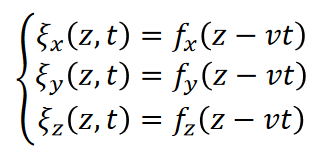
\includegraphics[width=0.4\textwidth]{screenshots/2024-04-10-09-26-33.png}
\end{figure}

\paragraph{Onde piane trasversali}
Rimandando all'esempio appena fatto, la condizione di onda trasversale si esprime tramite l'uguaglianza \(f_z(z-vt)\equiv 0\). In caso di direzione di propagazione \(\vec{\hat{u}}\), la condizione di onda trasversale è \(\vec{\hat{u}} \cdot \vec{f}(\vec{\hat{u}} \cdot \vec{r}-vt)=0\). Una componente quindi si annulla, mentre ne restano altre due indipendenti.
\begin{eg}
	[Onde trasversali comuni]
	Onde trasversali su corda elastica, onde elettromagnetiche, onde trasversali nei solidi (hanno velocità diverse da onde longitudinali), onde sismiche sussultorie (onde S, onde secondarie).
\end{eg}

\paragraph{Onde piane longitudinali}
Sempre pensando all'esempio precedente, se fosse un'onda longitudinale allora \(f_z(z-vt)\) dovrebbe essere l'unica componente diversa da zero. Le altre due componenti dovrebbero essere nulle. Quindi in generale la condizione di onda longitudinale rispetto a una direzione si esprime così: \(\vec{\hat{u}} \times \vec{f}(\vec{\hat{h}} \cdot \vec{r} - vt)\equiv \vec{0} \). Quindi rimane solo la componente nella direzione del moto.
\begin{eg}
	[Onde longitudinali comuni]
	Onde sonore, onde nel volume dei fluidi, onde longitudinali nei solidi, onde sismiche ondulatorie (onde P, onde principali).
\end{eg}

\section{Polarizzazione}
Nelle onde longitudinali non può esserci polarizzazione, alla fine sono analoghe alle onde scalari perché c'è una sola componente. Le trasversali hanno due componenti libere e quindi una dinamica più ricca.

\subsection{Primo caso: polarizzazione lineare}
Può capitare che le due componenti libere siano, a meno di una costante, la stessa funzione:
\begin{figure}[H]
	\centering
	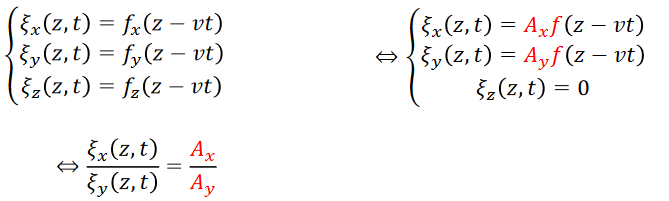
\includegraphics[width=0.6\textwidth]{screenshots/2024-04-10-09-37-47.png}
\end{figure}
Essendo le componenti x e y sempre proporzionali, il vettore \(\vec{\xi}(\vec{r},t)\) ha una direzione costante. Si può avere polarizzazione lineare sia per onde periodiche che impulsive.

\subsection{Polarizzazione circolare ed ellittica}
Consideriamo un caso particolare:
\begin{figure}[H]
	\centering
	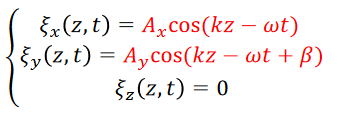
\includegraphics[width=0.4\textwidth]{screenshots/2024-04-10-09-41-16.png}
\end{figure}
Dobbiamo sviluppare un po' i calcoli per capire la relazione tra le componenti \(\xi _x\) e \(\xi _y\):
\begin{figure}[H]
	\centering
	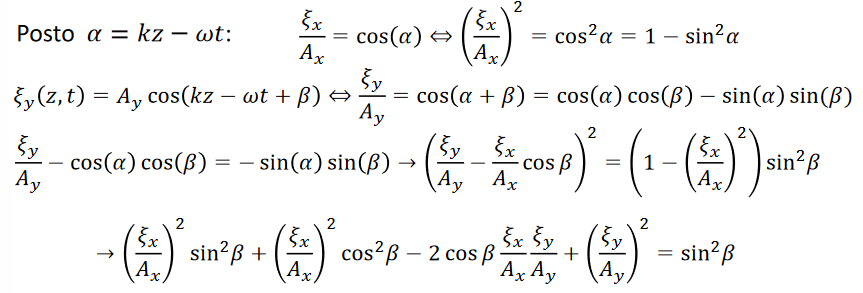
\includegraphics[width=0.6\textwidth]{screenshots/2024-04-10-09-43-52.png}
\end{figure}
Otteniamo un'equazione che non dipende nè dal tempo nè dallo spazio, in particolare è l'equazione di un ellisse!
\begin{equation}\label{eq:polarizzazione_ellittica}
	\left( \frac{\xi _x}{A_x} \right)^{2} +\left( \frac{\xi _y}{A_y} \right)^{2} -2 \cos \beta \frac{\xi _x}{A_x} \frac{\xi _y}{A_y} = \sin ^{2} \beta   
\end{equation}
\begin{figure}[H]
	\centering
	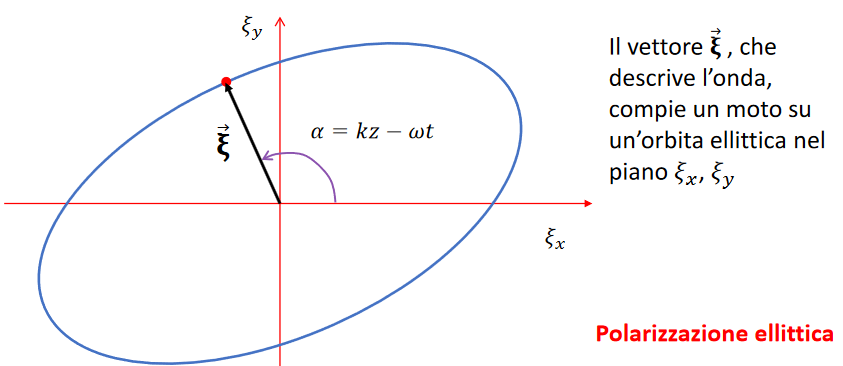
\includegraphics[width=0.6\textwidth]{screenshots/2024-04-10-09-48-32.png}
\end{figure}
Vediamo dei casi particolari.

\paragraph{Caso 1: \(\beta =0\)}
Ottengo
\begin{equation}
	\left( \frac{\xi _x}{A_x} \right)^{2} + \left( \frac{\xi _y}{A_y} \right)^{2} -2 \frac{\xi _x}{A_x}\frac{\xi _y}{A_y}=0 \rightsquigarrow 
	\left( \frac{\xi _x}{A_x}- \frac{\xi _y}{A_y} \right)^{2} =0 \rightsquigarrow 
	\frac{\xi _y}{A_y}=\frac{\xi _x}{A_x}   
\end{equation}
È esattamente la stessa situazione della polarizzazione lineare! Si tratta di un ellisse degenerato in una retta.

\paragraph{Caso 2: \(\beta = \pm \quotient{\pi }{2} \)}
L'equazione \eqref{eq:polarizzazione_ellittica} si riduce a
\begin{equation}
	\left( \frac{\xi _x}{A_x} \right)^{2} + \left( \frac{\xi _y}{A_y} \right)^{2} =1  
\end{equation} 
che è l'equazione di un ellisse con gli assi principali paralleli all'asse \(\xi _x\) e \(\xi _y\).
\begin{figure}[H]
	\centering
	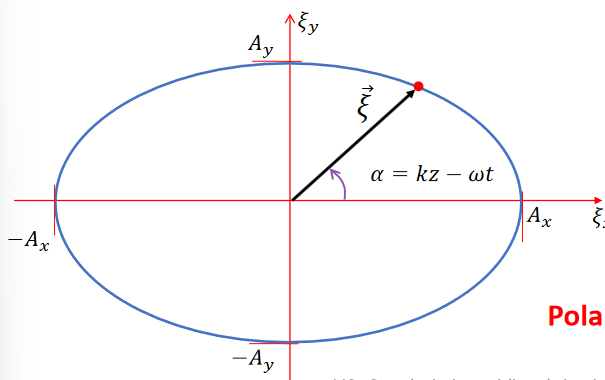
\includegraphics[width=0.5\textwidth]{screenshots/2024-04-10-09-55-50.png}
\end{figure}

\paragraph{Caso 3: \(\beta =\pm \quotient{\pi }{2},\ A_x=A_y \)}
L'equazione \eqref{eq:polarizzazione_ellittica} si riduce a quella di una circonferenza.
\begin{figure}[H]
	\centering
	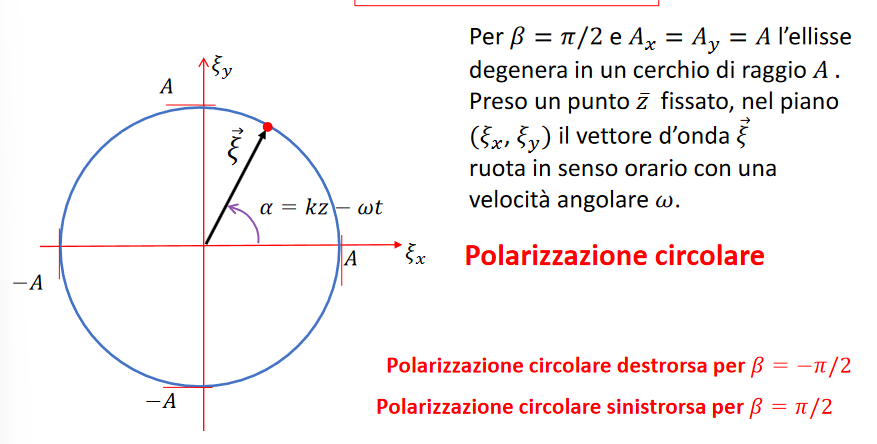
\includegraphics[width=0.7\textwidth]{screenshots/2024-04-10-09-57-37.png}
\end{figure}
In generale, il verso di rotazione si determina guardando l'onda che sta arrivando. Se, guardando arrivare l'onda, vedo il vettore ruotare in senso antiorario si parla di \emph{polarizzazione destrorsa}, altrimenti di \emph{polarizzazione sinistrorsa}. La polarizzazione destrorsa si avrà per \(-\pi \leq \beta \leq 0\), la polarizzazione sinistrorsa per \(0\leq \beta \leq \pi \). La polarizzazione è una relazione nello spazio tra le componenti di un'onda vettoriale, quindi si può verificare anche per le onde stazionarie!
\begin{remark}
	Quando si parla di polarizzazione ellittica non vale il principio di sovrapposizione! Devo avere \textbf{una sola onda armonica}. 
\end{remark}

\begin{note}
	Domanda tipica da orale: nella polarizzazione ellittica abbiamo la stessa pulsazione, ma vuol dire che siamo in una situazione di interferenza? No! Perché non sono sullo stesso asse.
\end{note}

\section{Principio di Huygens-Fresnel}
Qui in realtà non è necessario che l'onda sia vettoriale, quindi useremo le onde scalari per parlarne. Le onde sembrano propagarsi in linea retta, ma non è necessariamente vero! Ad esempio, noi sentiamo il suono anche se fra noi e la sorgente c'è un ostacolo. Stessa cosa vale per le onde elettromagnetiche. Marconi ha acceso una lampadina a New York dando il comando da Genova (che regaz). Anche le onde del mare, passando attraverso degli scogli, iniziano a propagarsi circolarmente invece che linearmente.

Questi fenomeni si descrivono bene attraverso il principio di Huygens-Fresnel, che è un "principio di classe B" perché in realtà è contenuto nelle equazioni di D'Alembert.
\begin{theorem}
	[Principio di Huygens-Fresnel]
	Ogni punto del fronte d'onda può essere considerato una nuova sorgente di onde sferiche, che si propagano in tutte le direzioni, con le stesse \(\nu \) e \(\omega \) dell'onda iniziale.
\end{theorem}
Noto un fronte d'onda al tempo t, si costruisce quello a \(t+ \mathrm{d} t\). Esempio:
\begin{figure}[H]
	\centering
	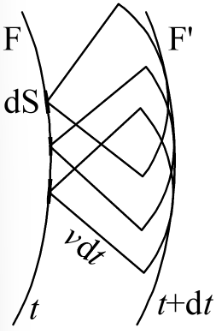
\includegraphics[width=0.3\textwidth]{screenshots/2024-04-10-10-24-36.png}
\end{figure}
Non devo solo conoscere il fronte d'onda, ma anche la direzione di moto del fronte d'onda. Mi serve quindi almeno un'informazione in più. Matematicamente scriviamo che
\begin{figure}[H]
	\centering
	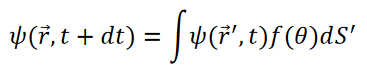
\includegraphics[width=0.4\textwidth]{screenshots/2024-04-10-10-26-15.png}
\end{figure}
Dove \(f(\theta )\) deve descrivere l'ampiezza al variare dell'angolo \(\theta \) nella figura seguente:
\begin{figure}[H]
	\centering
	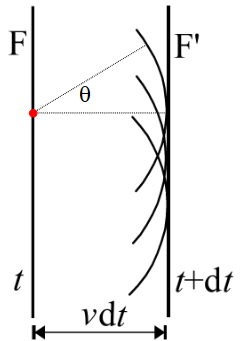
\includegraphics[width=0.3\textwidth]{screenshots/2024-04-10-10-27-25.png}
\end{figure}
Fresnel ipotizzò che \(f(\theta )= \frac{1}{2}(1+ \cos \theta )\). All'indietro così ho interferenza distruttiva. Applichiamola molto qualitativamente a un'onda piana:
\begin{figure}[H]
	\centering
	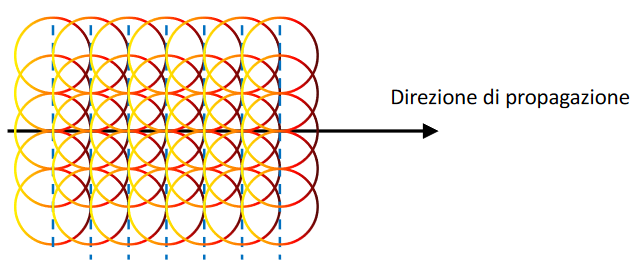
\includegraphics[width=0.5\textwidth]{screenshots/2024-04-10-10-28-36.png}
\end{figure}
In ottica geometrica, questo si traduce nel principio secondo cui l'angolo di incidenza di un raggio luminoso è uguale all'angolo di riflessione.
\begin{figure}[H]
	\centering
	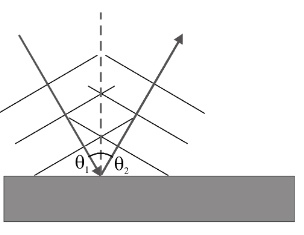
\includegraphics[width=0.4\textwidth]{screenshots/2024-04-10-10-31-33.png}
\end{figure}
Studiamo la motivazione fisica dietro a questo principio. Supponiamo che ci sia una parete infinita con un'apertura su cui arriva un'onda armonica piana scalare (per semplicità, altrimenti si applica alle tre componenti vettoriali). Sia l'onda \(\xi (z,t)=A \cos (kz-\omega t)=A \Re [e^{i(kz - \omega t)}]\). Sul piano \(\xi (0,t)= A \Re [e^{-i \omega t} ]\).
\begin{figure}[H]
	\centering
	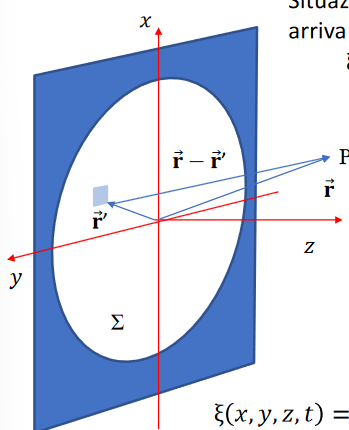
\includegraphics[width=0.4\textwidth]{screenshots/2024-04-10-10-34-16.png}
\end{figure}
Pongo \(s(x,y,z,t)= \vert \vec{r}-\vec{r}^{\prime} \vert \) e \(\cos \theta = \quotient{(\vec{r}-\vec{r}^{\prime} )\cdot \vec{\hat{k}}}{\vert \vec{r}-\vec{r}^{\prime} \vert } \). Applicando il principio si ottiene
\begin{figure}[H]
	\centering
	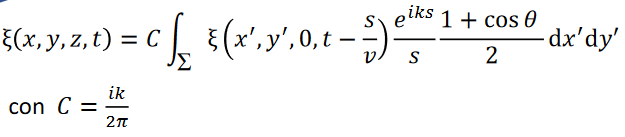
\includegraphics[width=0.5\textwidth]{screenshots/2024-04-10-10-37-37.png}
\end{figure}
\subsection{Limite dei piccoli angoli e diffrazione}
Se \(\vert \vec{r}^{\prime}  \vert \ll z \) possiamo trascurare la dipendenza angolare, ottenendo
\begin{figure}[H]
	\centering
	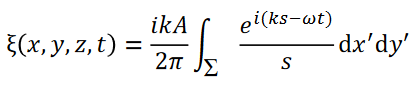
\includegraphics[width=0.4\textwidth]{screenshots/2024-04-10-10-39-02.png}
\end{figure}
Nel caso di onde non armoniche occorrerà chiaramente svilupparle in serie di Fourier. Scopriamo che le onde a lunghezza d'onda elevata saranno soppresse, quelle a lunghezza d'onda piccola rispetto all'apertura saranno poco deviate, mentre quelle con lunghezze d'onda confrontabili con l'apertura saranno quelle maggiormente deviate!

È la capacità delle onde di proseguire oltre gli ostacoli, eventualmente cambiando la forma del fronte d'onda!
\begin{figure}[H]
	\centering
	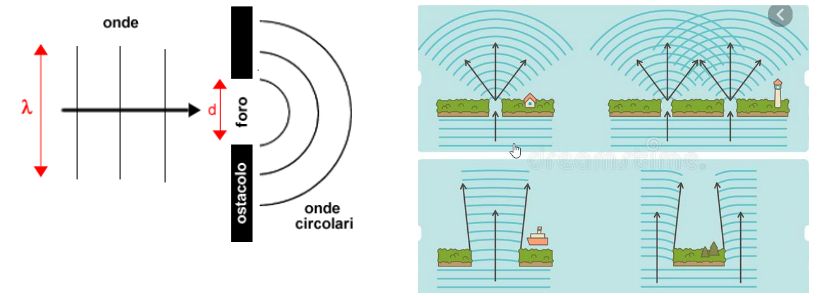
\includegraphics[width=0.6\textwidth]{screenshots/2024-04-10-10-43-31.png}
\end{figure}
Nell'immagine delle due aperture in alto a destra capiamo che le due onde genereranno interferenza perché hanno le stesse caratteristiche temporali.
Se ad esempio l'ostacolo che causa la diffrazione è un dischetto, sull'asse del disco avrò interferenza costruttiva e percepirò il segnale come se non ci fosse l'ostacolo.

Questi fenomeni avvengono anche con le onde sonore. In un generico punto dello spazio le onde sonore possono arrivare con una differenza di fase a causa della differenza nel percorso. Potrebbero addirittura avere intensità nulla!

\begin{note}
	Di questa lezione non sono importanti tanto i dettagli matematici quanto i concetti. L'integrale del principio di Huygens-Fresnel è molto complesso, quindi non ci sarà mai un esercizio in merito.
\end{note}